%%%%%%%%%%%%%%%%%%%%%%%%%%%%%%%%%%%%%%%%%%%%%%%%%%%%%%%%%%%%%%%%%%%%%%%%%%%%%%%%
% --------------------------------------------------- ADD APPENDIX (IN CASE) ---
%%%%%%%%%%%%%%%%%%%%%%%%%%%%%%%%%%%%%%%%%%%%%%%%%%%%%%%%%%%%%%%%%%%%%%%%%%%%%%%%
\appendix

\chapter{Determining the resolution of the detector types}
\label{sec:ResDetermination}


Two calibration spectra for the different kinds of detectors has been constructed using different gamma sources at various energies (see figure \ref{fig:Aufloesung})\cite{agostini_background_2017}.
From them two spectral resolution functions were able to be determined (see equation \ref{equ:BEGeCal} and \ref{equ:COAXCal}).
With these the resolution and therefore the full width at half maximum (FWHM) of a gamma line in the respective detector types can be determined only depending on the energy of the measured gamma.
Using these function the resolution of the detectors at the 514 keV line was determined to be $\Delta E_{\mathrm{BEGe}}] =2.26706\unit{keV}$ for the BEGe and $\Delta E_{\mathrm{COAX}}] = 2.72196\unit{keV}$ for the COAX detectors.



\begin{equation}
\Delta E_{BEGe}(x[keV]) = 2.35482 \times \sqrt{0.7065+0.0004286x}
\label{equ:BEGeCal}
\end{equation}

\begin{equation}
\Delta E_{COAX}(x[keV]) = 2.35482 \times \sqrt{1.01314+0.0006284x}
\label{equ:COAXCal}
\end{equation}
\\

For the fit process it is also of interest to know the value of the expected variance $\sigma$ of the Gaussian peak functions.
With the FWHM this can easily be calculated by applying function \ref{equ:sigma}.

\begin{equation}
\sigma (\Delta E) = \frac{\Delta E}{2\sqrt{2\ln2}}
\label{equ:sigma}
\end{equation}

By applying this function one results in $\sigma_{BEGe} = 0.96273\unit{keV}$ and $\sigma_{COAX} = 1.15591\unit{keV}$ at an energy of 514 keV.

\begin{figure}
	\centering
	\ifmakefigures%
	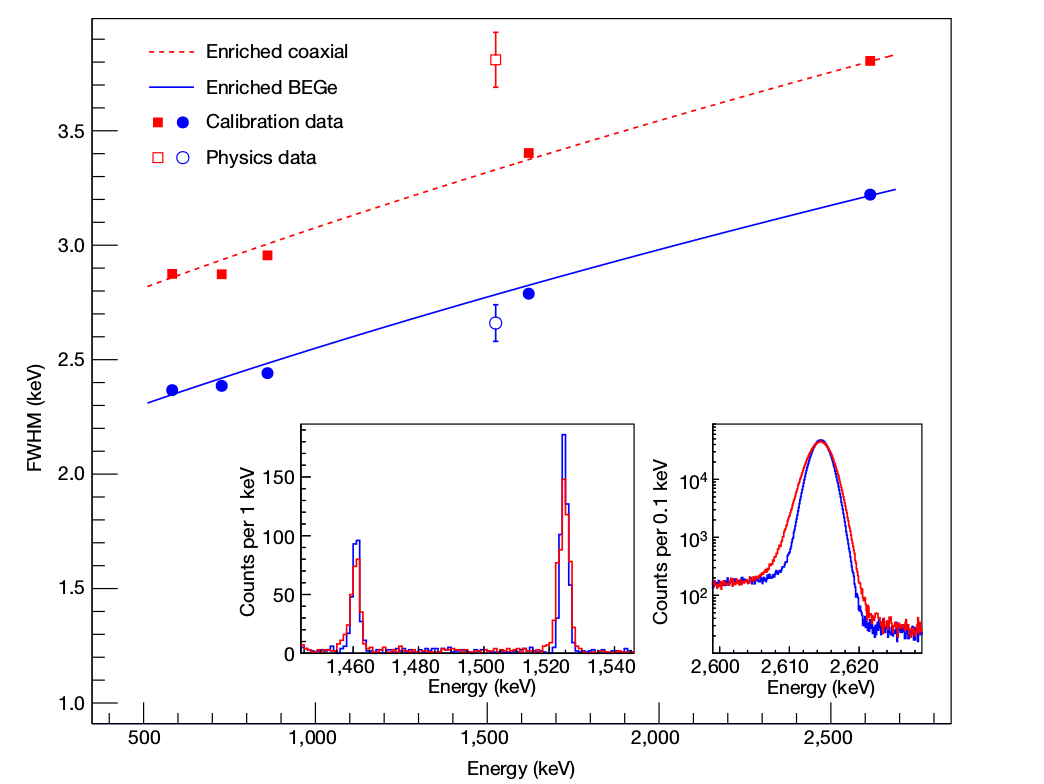
\includegraphics[width=80mm]{./Bilder/Aufloesung.png}
	\fi%
	\caption{
		The full width at half maximum (FWHM) of a investigated gamma lines in the respective detectors as a function of the energy of the investigated gamma.
		This value corresponds to the average resolution of the detectors at the respective energies.
		Taken from \cite{agostini_background_2017}.
	}
	\label{fig:Aufloesung}
\end{figure}


\chapter{Detector Overview}

In the second method to determine the specific \Kr\ activity in the LAr of \gerda\ \PII\ only the data of those detectors was used that have been turned on over the entire time inspected.


\begin{table}
	\begin{tabular}{|l|l|r|r||l|l|r|r|}
		\hline
		Number & Type & on from 53-92 & 55-92 & Number & Type & on from 53-92 & 55-92 \\
		\hline
		0 & BEGe & X & X & 20 & BEGe & X & X \\
		\hline
		1 & BEGe & X & X & 21 & BEGe & X & X \\
		\hline
		2 & BEGe & X & X & 22 & BEGe & X & X \\
		\hline
		3 & BEGe &  & X & 23 & BEGe &  &  \\
		\hline
		4 & BEGe &  & X & 24 & BEGe & X & X \\
		\hline
		5 & BEGe &  &  & 25 & BEGe &  & X \\
		\hline
		6 & BEGe &  &  & 26 & BEGe &  &  \\
		\hline
		7 & BEGe &  &  & 27 & COAX &  &  \\
		\hline
		8 & COAX &  & X & 28 & COAX &  & X \\
		\hline
		9 & COAX &  & X & 29 & COAX & X & X \\
		\hline
		10 & COAX & X & X & 30 & BEGe & X & X \\
		\hline
		11 & BEGe & X & X & 31 & BEGe &  & X \\
		\hline
		12 & BEGe &  & X & 32 & BEGe &  &  \\
		\hline
		13 & BEGe &  &  & 33 & BEGe &  &  \\
		\hline
		14 & BEGe & X & X & 34 & BEGe & &  \\
		\hline
		15 & BEGe &  &  & 35 & BEGe &  &  \\
		\hline
		16 & BEGe &  &  & 36 & COAX &  &  \\
		\hline
		17 & BEGe & X & X & 37 & natural &  &  \\
		\hline
		18 & BEGe &  & X & 38 & natural &  &  \\
		\hline
		19 & BEGe & X & X & 39 & natural &  &  \\
		\hline
	\end{tabular}
\end{table}

\begin{figure}
	\centering
	\ifmakefigures%
	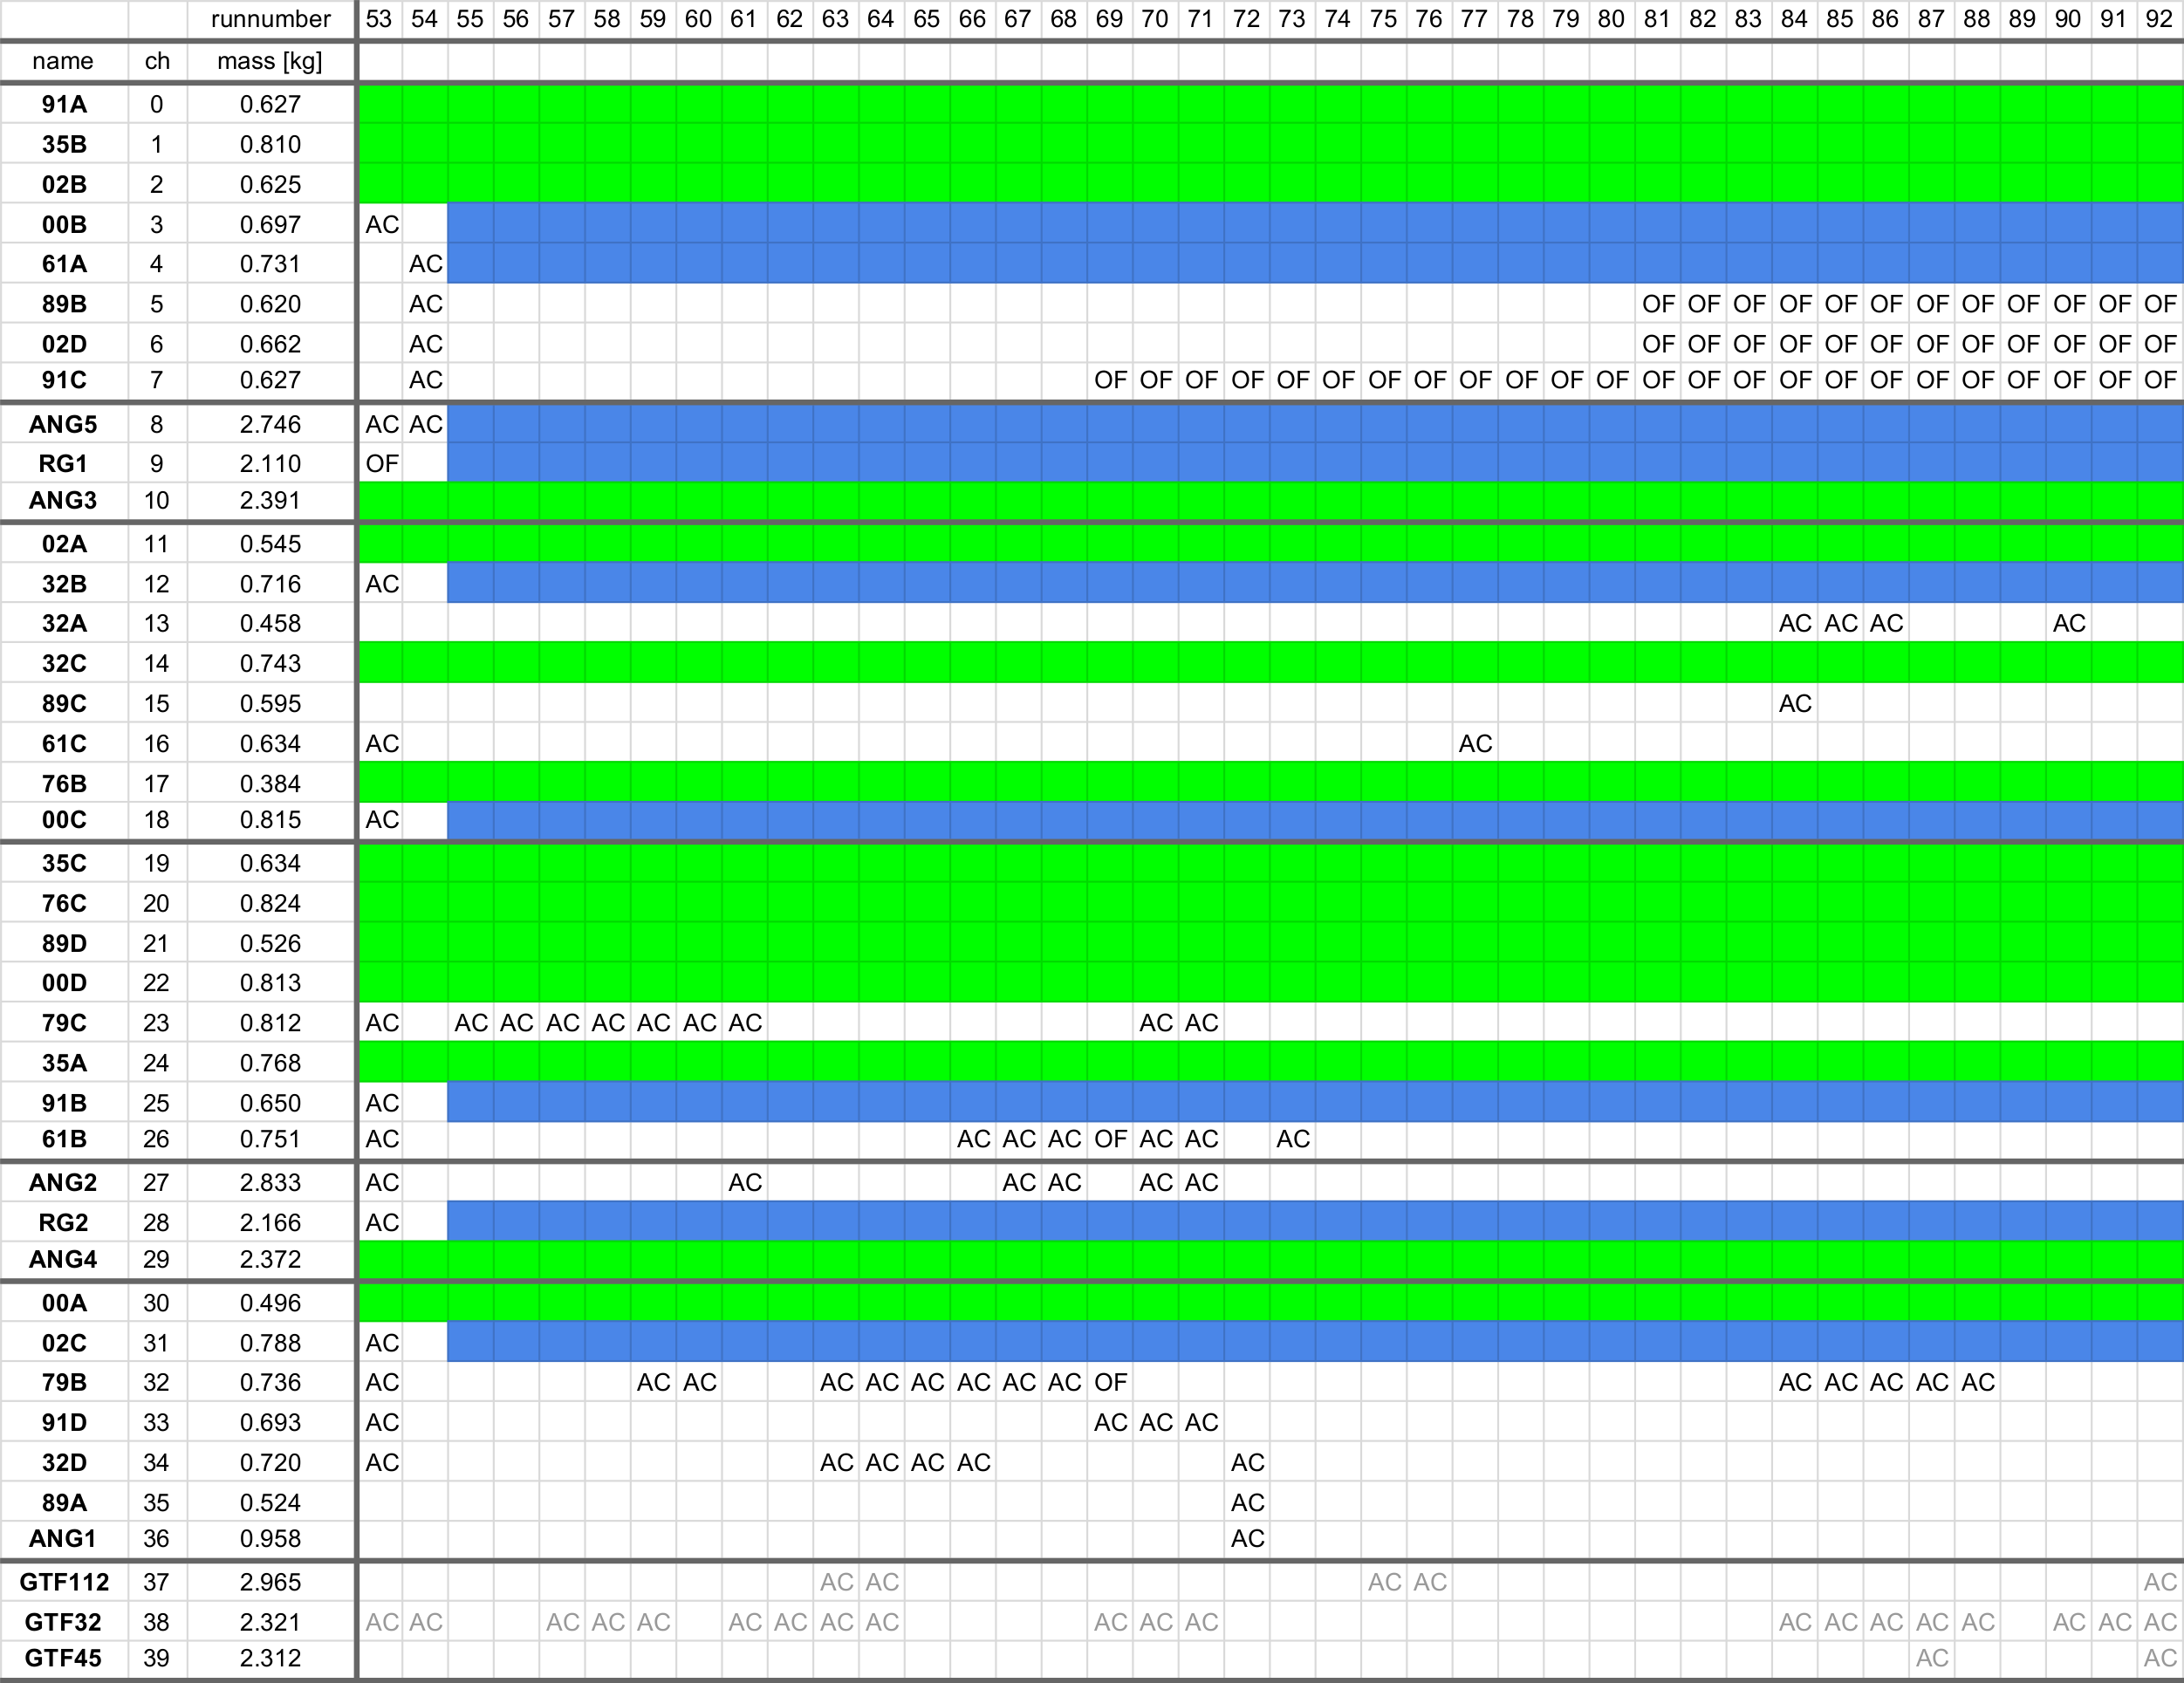
\includegraphics[width=80mm]{./Bilder/runOverview.png}
	\fi%
	\caption{
		The full width at half maximum (FWHM) of a investigated gamma lines in the respective detectors as a function of the energy of the investigated gamma.
		This value corresponds to the average resolution of the detectors at the respective energies.
		Taken from \cite{agostini_background_2017}.
	}
	\label{fig:Aufloesung}
\end{figure}

% \section{}
% \label{}
